

L'étude proposée porte sur la réplique terrestre\footnote{Utilisée sur Terre pour validation des différents sous-systèmes.} du
système InSIGHT (\textbf{In}terior exploration using \textbf{S}eismic
\textbf{I}nvestigations, \textbf{G}eodesy and \textbf{H}eat
\textbf{T}ransport), projet du CNES (Centre National d'Études Spatiales)
qui a pour but de déployer une station d'étude de la structure interne
de la planète Mars.





\begin{figure}[!htb]
\begin{center}
\begin{minipage}{0.55\textwidth}
le sous-système SEIS (figure\ref{fig2}) sera l'objet de l'étude proposée. Il est
basé sur un instrument hybride composé :

\begin{itemize}
\item
  d'un système de déploiement (DPL) ;
\item
  d'une sphère comportant trois capteurs sismiques à très larges bandes
  et leurs capteurs de température. La sphère dispose d'un système de
  référencement de ses pieds (\textbf{figure 3}). Sa masse est d'environ
  3 kg et sa consommation électrique varie autour de 1W.
\item
  d'une boîte électronique d'acquisition dont la structure est donnée
  par le diagramme de définition des blocs de la figure \ref{fig4}.
\end{itemize}
\end{minipage}
\begin{minipage}{0.45\textwidth}
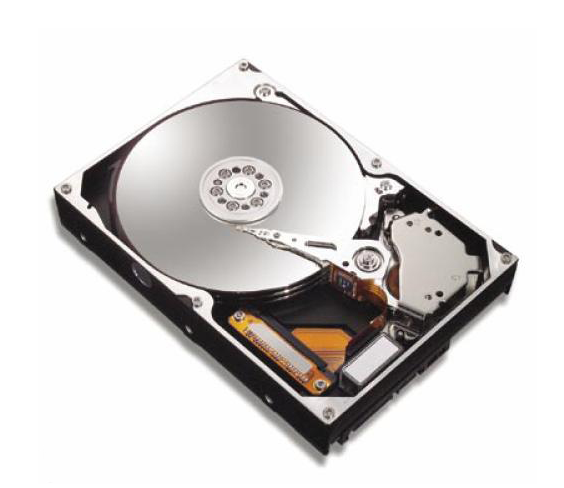
\includegraphics[width=0.8\textwidth]{image2.png}
\caption{Ensemble SEIS en phase de déploiement \label{fig2}}
\end{minipage}
\end{center}
\end{figure}

\begin{obj}
Ecrire un programme permettant de gérer les
signaux de commandes des pieds du SEIS pour le maintenir en position à
partir de mesures réalisées par des capteurs de position à ultrasons.
\end{obj}

\begin{figure}[!htb]
\begin{center}
\begin{minipage}{0.55\textwidth}
Dans cette partie on s'intéresse à la génération de la consigne de position à appliquer à chacun de ces pieds via un micro-controleur (type carte arduino).
\end{minipage}
\begin{minipage}{0.45\textwidth}
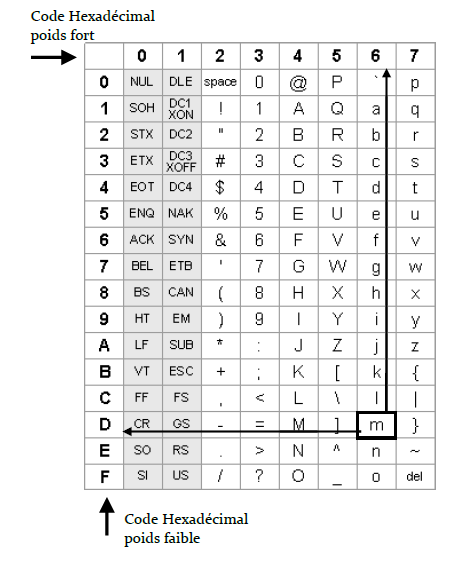
\includegraphics[width=0.8\textwidth]{image14.png}
\caption{Carte Arduino Uno \label{fig3}}
\end{minipage}
\end{center}
\end{figure}


On dispose d'une carte Arduino Uno qui peut être programmée dans
différents langages. \textbf{On se limitera à l'utilisation du
langage de programmation Python pour l'étude proposée}.

Le calculateur (la carte Arduino dans notre cas), qui contrôle le
mouvement des trois vérins électriques, génère, pour chaque vérin, un
signal de consigne rapide (vitesse maximale du moteur) ou lent (un
dixième de la vitesse maximale du moteur) en fonction de l'avance de
celui-ci. Dans une première phase, il génère une consigne dite « rapide
» jusqu'à atteindre une distance de 10 mm entre la tige du vérin et le
sol. Le système de commande délivre alors une consigne dite « lente »
afin de limiter les contraintes lors du contact entre chaque vérin et le
sol. Lors de cette deuxième phase (consigne « lente »), un
asservissement en position de chaque vérin permet de maintenir le
châssis du SEIS en position horizontale par rapport au sol.

On note pour la suite de l'étude (\textbf{figure \ref{fig15}}) :

\begin{itemize}
\item
  \pyv{distance} : la variable, de type float, correspondant à la
  distance mesurée entre le sol et le capteur donnée en cm ;
\item
  \pyv{distance_verin} : la variable, de type float, correspondant à
  la distance entre le capteur et l'extrémité de la tige du vérin donnée
  en cm ;
\item
  \pyv{rapide} et \pyv{lente} : variable globale avec des valeurs
  prédéfinies (correspond aux consignes de la commande du vérin électrique : vitesse rapide, vitesse lente).
\end{itemize}


\begin{figure}[!htb]
\begin{center}
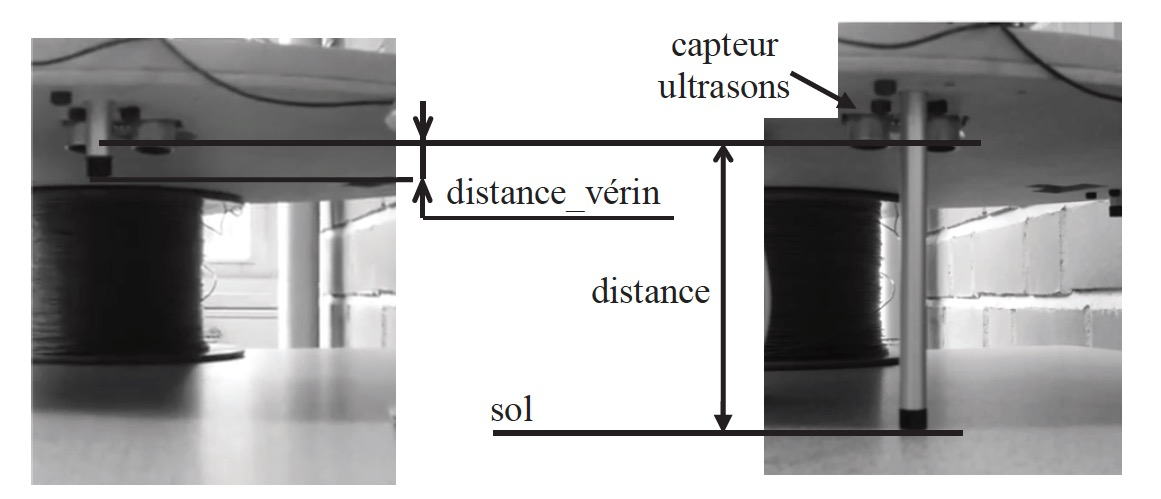
\includegraphics[width=0.8\textwidth]{image15.jpg}
\caption{Sortie du vérin 1 \label{fig15}}
\end{center}
\end{figure}


\question{Écrire une fonction \pyv{consigne(distance,distance\_verin)} qui calcule l'écart entre la
tige du vérin et le sol et qui retourne la consigne \pyv{rapide} si
cet écart est supérieur à 10 mm ou la consigne \pyv{lente} sinon.}

Le module SEIS est équipé de trois
capteurs de positions, à ultrasons, associés à chaque vérin électrique.
Chaque capteur est constitué d'un émetteur et d'un récepteur à
ultrasons. Le principe de mesure des capteurs à ultrasons utilisés est
donné ci-dessous et illustré sur la \textbf{figure \ref{fig16}}.

Pour déclencher une mesure, il faut présenter une impulsion « High » (5
V) d'au moins 10 $\mu s$ sur l'entrée « Trig » du capteur (sortie de la carte
Arduino). L'émetteur à ultrasons délivre alors une série de 8 impulsions
ultrasoniques à 40 kHz, puis il attend le signal réfléchi. Lorsque
celui-ci est détecté par le récepteur à ultrasons, le capteur impose un
signal « High » sur la sortie « Echo » (entrée de la carte Arduino) dont la durée, tc, est proportionnelle à la distance
mesurée. La distance est obtenue en

multipliant la durée du signal tc en seconde par le coefficient constant
17 150 pour obtenir la valeur de la distance en cm.
\begin{figure}[!htb]
\begin{center}
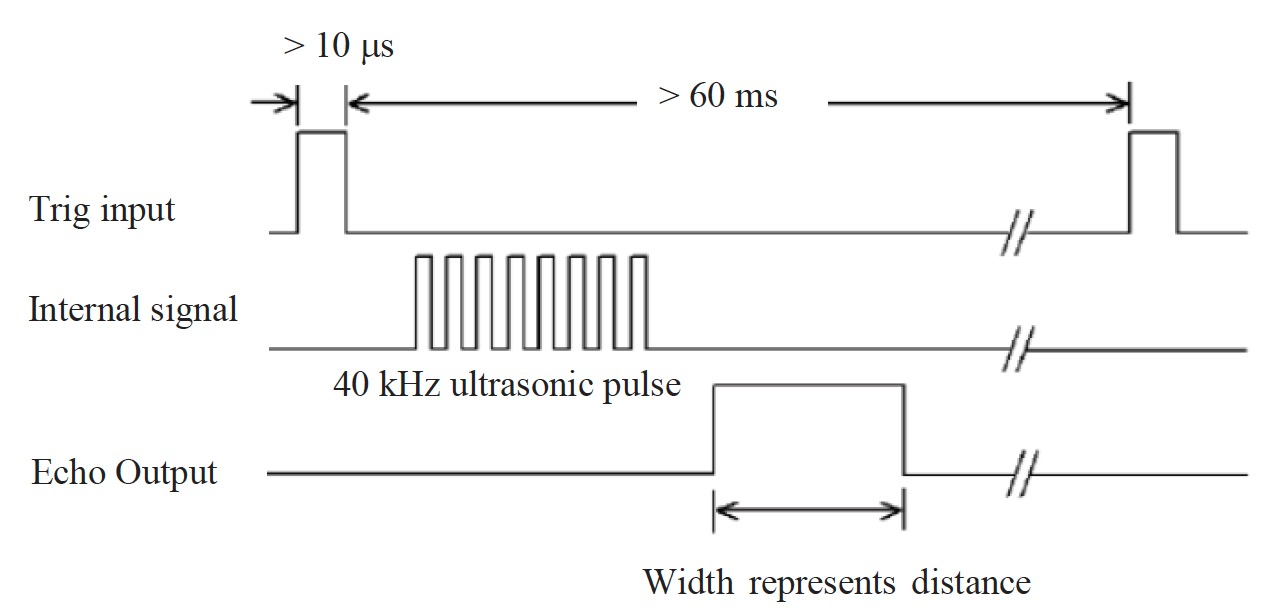
\includegraphics[width=0.8\textwidth]{image18.jpg}
\caption{Séquence des signaux permettant une mesure  \label{fig16}}
\end{center}
\end{figure}